\newcommand{\PFF}[1]{./body/aux/principles/#1}
\def\checkmark{\tikz\fill[scale=0.4](0,.35) -- (.25,0) -- (1,.7) -- (.25,.15) -- cycle;}
\def\ccross{\tikz\draw[scale=0.3, thick] (0.4, 0.4) -- (-0.4, -0.4) (0.4, -0.4) -- (-0.4, 0.4);}
\documentclass[../ml-tct.tex]{subfiles}
\begin{document}
\chapter{Principles of \xray\ \texorpdfstring{\gls{ct}}{Computed Tomography}}%
\label{chap:principles}
\myepigraph{I did not think, I investigated.}{Wilhelm Röntgen}{McClure's Magazine VI No. 5, 1896}

\minitoc%
Modern medicine relies greatly on imaging techniques, where different physical processes are exploited to give insights into the human body.
For instance, \gls{mri} measures proton density with the help of strong magnetic fields, field gradients and radio pulses, by which an excellent soft-tissue contrast can be achieved.
The importance of \gls{mri} in medicine is emphasized by the \DTMfetchyear{mri-nobel} \nobelprice, which was awarded to Peter Mansfield and Paul Lauterbur \enquote{for their discoveries concerning magnetic resonance imaging}\footnote{see \url{https://www.nobelprize.org/prizes/medicine/2003/summary/}, accessed \DTMDisplaydate{2021}{04}{19}{-1}}.

\xray\ \gls{ct} is of similar importance in modern medicine, where by help of ionizing radiation cross-sections of the body are imaged with great hard-tissue contrast.
In \DTMfetchyear{ct-nobel}, Allan Cormack and Godfrey Hounsfield were rewarded the \nobelprice\ \enquote{for the development of computer assisted tomography}\footnote{see \url{https://www.nobelprize.org/prizes/medicine/1979/summary/}, accessed \DTMdisplaydate{2021}{04}{19}{-1}}.
Practically, the advantages of \gls{ct} over \gls{mri} are the reduced costs in both acquisition and operation, as well as faster image acquisition.
The main disadvantage is the usage of ionizing radiation, whose energy fundamentally must be at least partly deposited in the body to create contrast.

In the following sections, we will outline the principles of \xray\ \gls{ct}.
We will define the tomography problem, go over physical principles and instrumentation in \gls{ct}, and will build the mathematical foundation needed in the next chapters along the way.
Since our focus is on reconstruction, we refer the reader to~\cite{buzug_computed_2008,prince_medical_2014} for a more in-depth review of the physics of \gls{ct}.
\section{Tomography}
In the most general sense, \emph{tomography} describes the \enquote{imaging of cross-sections}.
The word is derived from the Greek words \transexpl{τόμος}{tomos}{\enquote{slice} or \enquote{section}} and \transexpl{γράφω}{graphō}{\enquote{to write} or \enquote{to describe}}.
Specifically, given some volume, we are interested in visualizing distinct slices with minimal interference of the rest of the volume.
This is distinctly different from projectional methods, where the resulting two-dimensional projection displays information of the volume integrated over a specific direction.
We show an example illustrating the difference between tomography and projectional imaging in~\cref{fig:principles:tomo vs proj}.
\begin{figure}
	\centering
	\includestandalone[width=\textwidth]{\PFF{tomo-proj}}
	\caption[Tomography versus projectional imaging.]{%
		Tomography versus projectional imaging:
		In tomography, the goal is to acquire the cross sections shown in red, whereas in projectional imaging, a specific direction is integrated over.
	}%
	\label{fig:principles:tomo vs proj}
\end{figure}

Besides medical applications, where the body of interest is (a specific part of) the human body, tomography is widely used in the geosciences, where the body of interest is (a specific part of) the earth.
As an example, in seismic tomography, seismographs across the earth's surface register motion of the ground induced by earthquakes.
With this information, certain characteristic of the rock can be reconstructed~\cite{nolet_seismic_1987}.
In muon tomography, muons from cosmic radiation are used to image large-scale structures.
This has been used to image the reactor after the \DTMfetchyear{fukushima} Fukushima Daiichi nuclear disaster, to assess the situation of the remains of the reactor cores~\cite{borozdin_cosmic_2012}.
\section{Physical Principles}
The underlying physical principle of \xray\ \gls{ct} and \xray\ projection radiography is attenuation of electromagnetic radiation by any given medium.
The term \enquote{\xray} itself describes a specific interval in the electromagnetic spectrum, which is of high enough energy to be classified as \emph{ionizing} radiation.
Ionizing radiation, as opposed to non-ionizing radiation, is capable of ejecting electrons from atoms and thereby creating ions.
It is the interaction between ionizing radiation, most often produced by the \xray\ tube, and the atoms of the patient's body that ultimately yield the contrast in the \xray\ image.
\subsection{Electromagnetic Radiation}
Classically, electromagnetic radiation describes waves of the electromagnetic field propagating through space.
An electromagnetic wave consists of an electric and a magnetic component, which are perpendicular to each other.
The relationship between the electric and magnetic component is described by the famous Maxwell's equations.
We schematically show the propagation of a linearly polarized electromagnetic wave with wavelength \( \lambda \) in~\cref{fig:principles:wave prop}.
\begin{figure}
	\centering
	\includestandalone[width=\textwidth]{\PFF{waveprop}}
	\caption[Propagation of an electromagnetic wave.]{%
		The propagation of an electromagnetic wave:
		The electric field \( E \) is perpendicular to the magnetic field \( B \).
		The direction of propagation is referred to as the wave number \( k \).
	}%
	\label{fig:principles:wave prop}
\end{figure}
The wavelength of a electromagnetic wave is related to its frequency by
\begin{equation}
	\nu = \frac{\si{\clight}}{\lambda}
\end{equation}
with the speed of light \( \si{\clight} = \SI{3e8}{\meter\per\second} \).

The particles associated with electromagnetic radiation are referred to as \emph{photons}.
The energy of a photon associated with a wave of frequency \( \nu \) is
\begin{equation}
	E = h \nu,
\end{equation}
where \( h = \SI{6.62607015e-34}{\joule\second} \) is Planck's constant.
Electromagnetic waves exist on an energy spectrum, where different classes are defined.
Radio waves, visible light and \xray{}s are examples of electromagnetic radiation, with radio waves having the lowest energy of the three.
For medical radiography applications, radiation in the range of \SIrange{25}{500}{\kilo\electronvolt} is used.

We show the electromagnetic spectrum with some important classes in~\cref{fig:principles:spectrum}.
\begin{figure}
	\centering
	\includestandalone[width=\textwidth]{\PFF{spectrum}}
	\caption[The electromagnetic spectrum with commonly distinguisehd classes.]{%
		The electromagnetic spectrum with some frequently distinguished energy ranges.
		The slanted line should emphasize that \xray{}s and Gamma rays are distinguished by their point of origin rather than their energy, and that there some overlap in energy.
	}%
	\label{fig:principles:spectrum}
\end{figure}
We note that, although \xray{}s and Gamma rays are usually distinct classes in the electromagnetic spectrum, they are not distinguished by energy but by point of origin.
Specifically, \xray{}s are defined as radiation originating from the electron cloud, while gamma rays originate from the nucleus of an atom.
\subsection{Interactions of Electromagnetic Radiation with Matter}
Ionizing electromagnetic radiation interacts with matter primarily by
\begin{enumerate*}
	\item the photoelectric effect,
	\item Compton scattering, and
	\item pair production.
\end{enumerate*}
Typically, pair production is only considered relevant for high energy photons with \( E > \SI{1.022}{\mega\electronvolt} \).
As previously mentioned, in the medical imaging domain the highest energies are approximately \SI{500}{\kilo\electronvolt} and as such pair production can largely be neglected.
For both the photoelectric effect and Compton scattering, the interaction of the \xray\ with the atoms happens in the electron shell.
The defining difference between the photoelectric effect and Compton scattering is that in the latter (the energy of) the photon is not fully absorbed by the atom.
In medical imaging, the contrast is mostly due to the photoelectric effect, whereas Compton scattering limits the resolution of the images.
We show the three interaction mechanisms schematically in~\cref{fig:principles:em interaction}.
\begin{figure}
	\centering
	\begin{subfigure}{0.3\textwidth}
		\centering%
		\includestandalone[width=\textwidth]{\PFF{interaction_photoelectric}}
		\caption{Photoelectric Effect}%
		\label{fig:principles:em interaction:photo}
	\end{subfigure}\hfill%
	\begin{subfigure}{0.3\textwidth}
		\centering
		\includestandalone[width=\textwidth]{\PFF{interaction_compton}}
		\caption{Compton Effect}%
		\label{fig:principles:em interaction:compton}
	\end{subfigure}\hfill%
	\begin{subfigure}{0.3\textwidth}
		\centering
		\includestandalone[width=\textwidth]{\PFF{interaction_pair}}
		\caption{Pair Production}%
		\label{fig:principles:em interaction:pair}
	\end{subfigure}%
	\caption[Interactions between electromagnetic radiation and matter.]{%
		Illustration of the three principles of interaction between electromagnetic radiation and matter.
		The wavelength of the incident ray indicates the relative energies that these effects are most likely to occur at.
		Pair Production only happens for \( E > \SI{1.022}{\mega\electronvolt} \), and as such can largely be ignored for medical applications.
	}%
	\label{fig:principles:em interaction}
\end{figure}
\subsubsection{Photoelectric Effect}
In the photoelectric effect, through interaction of a photon with the coulomb field of the nucleus, an electron from an inner shell, most often the K-shell, is ejected from the atom.
The incident photon of energy \( E_p = h\nu_p \) is fully absorbed by the atom, and the electron is ejected with energy
\begin{equation}
	E_{e^-} = E_p - E_B,
\end{equation}
where \( E_B \) is the binding energy of the electron.
The hole of the ejected (usually K-shell) electron is then filled by an electron in an outer shell.
The energy difference between the shells is converted into electromagnetic radiation (\xray{}s), which is characteristic to the atom, as the structure of the atom dictates the energy delta between the shells.

The resulting characteristic \xray{}s may sometimes eject another outer-shell electron, called the \emph{Auger electron}, and consequently lead to readjustment of the remaining electrons.
The ejected electrons (photoelectrons and Auger electrons) can then be treated as typical particulate radiation, and interact with the matter around them.
In fact, these particles contribute largely to the biological effects of ionizing radiation.
We show an illustration of the photoelectric effect (without considering Auger electrons) in~\cref{fig:principles:em interaction:photo}.
\subsubsection{Compton Scattering}
In contrast to the photoelectric effect, in Compton scattering the energy \( E_p = h\nu_p \) of the incident photon is not fully absorbed by the atom.
Instead, it loses some energy in the process of ejecting an outer-shell electron (the \emph{Compton electron}), and is deflected by the \emph{Compton angle} \( \theta \).
These concepts are illustrated in~\cref{fig:principles:em interaction:compton}.
Depending on the Compton angle \( \theta \), the energy \( E_c \) of the \emph{Compton photon} is given by
\begin{equation}
	E_c = \frac{E_p}{1 + (1 - \cos \theta)\frac{ E_p}{\si{\electronmass\clight^2}}}
\end{equation}
where \( \si{\electronmass\clight^2} = \SI{511}{\kilo\electronvolt} \) is the rest energy of an electron.
We see that the Compton photon has the smallest energy when \( \theta = \pi\,\mathrm{rad} \), i.e.\ when the photon is reflected back to the incidence direction.
The ejected electron is again free to interact with the surrounding matter.
\subsubsection{Pair Production}
Although not interesting for medical applications, we briefly discuss pair production here for completeness.
Pair production is the primary principle of interaction of high-energy photons with matter.
Specifically, incident photons with \( E_p > \SI{1.022}{\mega\electronvolt} \), or \( \lambda < \SI{1.2132}{\pico\meter} \), may \enquote{decay} into an electron-positron pair when near a nucleus.
The requirements are very specific:
The energy for such interactions is bounded from below with \SI{1.022}{\mega\electronvolt}, as this is the rest energy \( 2 \si{\electronmass\clight^2} \) of an electron-positron pair.
Further, the decay event must happen near a nucleus, as otherwise conservation of momentum would necessarily need to be violated.
As a result, the nucleus typically experiences some \enquote{recoil} during such events.
The electron and positron are then free to interact with their neighborhood.
The most likely fate of the positron is an electron-positron annihilation event, which can be thought of as the inverse of pair production.
\subsection{Attenuation of Electromagnetic Radiation in Matter}
In the previous sections, we described the primary principles by which electromagnetic radiation can interact with matter.
Here, we want to consider these effects on a macroscopic level.
We do this by introducing probabilistic concepts modeling the effects on a macroscopic level.
With simplified examples, we finally arrive at a signal model in dependence of the quantity of interest, which is the attenuation coefficient of the imaged body.

\subsubsection{Probabilities of Interaction}
Let us first informally consider the probabilities of the different interactions of electromagnetic radiation with matter.
The photoelectric effect requires interaction with the Coulomb field of the nucleus of an atom.
Consequently, the probability of a photoelectric event is related to the atomic number \( \atomicnumber \) of an atom.
In a heterogeneous material composed of different elements, we define the effective atomic number \( \effectiveAN \), which summarizes the compound.
The probability of a photoelectric event is \( \propto \effectiveAN^4 \) for the compounds typically found in human tissue.
Further affecting the probability of photoelectric events is the energy of the incident ray, such that in summary \( \prob{\text{PE event}} \propto \frac{\effectiveAN^4}{{(h\nu)}^3} \).
The binding energy of the inner shell electrons also affects the probability of photoelectric events, which is exploited in contrast agents.

Compton scattering on the other hand describes an interaction with outer, loosely bound electrons.
The probability of Compton events is mainly dependent on the electron density in the material, i.e. \( \prob{\text{CS event}} \propto \frac{\avogadro \atomicnumber}{\molweight} \).
Here, \( \avogadro = \SI{6.02214076e23}{\per\mole} \) is Avogadro's constant, and \( \molweight \) is the molecular weight in \si{\gram\per\mole}.
In human tissue, the electron density does not vary hugely, with it being around \SI{3.1e26}{\per\kilo\gram}~\cite{wolbarst_physics_2005} for air, water, muscle, fat and bone.
Therefore, the probability of Compton events is largely independent of the atomic number.
Also, according to the Klein-Nishina formula~\cite{klein_scattering_1994}, the probability for Compton events in the energy range for medical applications is close to constant.

We show the relative frequency of occurrence between Compton and photoelectric events in~\cref{tab:pe vs cs} (adapted from~\cite{johns_physics_2014}).
\begin{table}
	\centering
	\caption[Relative impact of interactions for different energies in water.]{%
		Relative impact of Compton Scattering versus the photoelectric effect for different photon energies in water.
		Adapted from~\cite{johns_physics_2014}.
	}%
	\label{tab:pe vs cs}
	\begin{tabular}{SSS}
		{Photon Energy in \si{\kilo\electronvolt}} & {Compton Interactions in \si{\percent}} & {Energy Transfer by CS in \si{\percent}}\\
		\toprule
		20 & 26.4 & 1.3 \\
		40 & 77.9 & 19.3 \\
		60 & 93.0 & 55.0 \\
		80 & 97.0 & 78.8 \\
		100 & 98.4 & 89.6 \\
		150 & 99.5 & 97.4 \\
		400 & 99.9 & 99.9 \\
		\bottomrule
	\end{tabular}
\end{table}
It shows that in the energy range that is interesting for medical applications, except for the lower end, Compton scattering is the dominating modus of interaction in terms of number of occurrences.
The share Compton scattering increases with increasing photon energy, where at \( E_p = \SI{60}{\kilo\electronvolt} \) Compton scattering accounts for \SI{93}{\percent} of all interactions.
However, since in a Compton scattering event the energy is only partly deposited in the atom, it accounts for \SI{55}{\percent} of the deposited energy at \SI{60}{\kilo\electronvolt}.
For energies \( > \SI{60}{\kilo\electronvolt} \), Compton scattering also quickly becomes the dominating mode of energy transfer.
\subsubsection{Monochromatic Narrow Beam and Homogeneous Thin Slab}
To build up a signal model, we will consider the following setup:
From some source, \( N \) photons with the same energy are shot perpendicularly onto a thin, homogeneous slab of thickness \( \Delta x \).
Behind the slab is a \enquote{perfect} detector with the same footprint as the incident beam.
Clearly, without the slab we would expect the detector to count \( N \) photons.
The slab however will absorb some photons by the photoelectric effect, as well as scatter photons by Compton scattering events such that they are no longer counted by the detector.
In general, the detector will count \( N^\prime < N \) photons, i.e.\ the slab has \emph{attenuated} the photon beam.
We show the narrow beam geometry along with the distinctly different broad beam geometry in~\cref{fig:principles:beam geometries}.
\begin{figure}
	\centering
	\begin{subfigure}{0.45\textwidth}
		\centering%
		\includestandalone[width=\textwidth]{\PFF{narrow_beam}}
		\caption{Narrow Beam}%
		\label{fig:principles:geometry:narrow}
	\end{subfigure}\hfill%
	\begin{subfigure}{0.45\textwidth}
		\centering
		\includestandalone[width=\textwidth]{\PFF{broad_beam}}
		\caption{Broad Beam}%
		\label{fig:principles:geometry:broad}
	\end{subfigure}%
	\caption[Beam geometries: Narrow versus Broad Beam.]{%
		The narrow beam geometry~\subref{fig:principles:geometry:narrow}, where the footprint of the detector is as large as the incident beam, is a simple model for studying attenuation.
		If the incident beam is broader than the detector~\subref{fig:principles:geometry:broad}, it may pick up scattered photons.
	}%
	\label{fig:principles:beam geometries}
\end{figure}

We denote with \( \Delta N = N - N^\prime \) the difference between the number of incident and detected photons.
Assuming \( \Delta x \) is small, we expect \( \Delta N \) to be proportional to both \( \Delta x \) and \( N \), i.e.
\begin{equation}
	\Delta N = \mu N \Delta x,
\end{equation}
where \( \mu \) is the (material dependent) proportionality constant, known as the \emph{linear attenuation coefficient}.
For the sake of simplicity, we treat \( N \) as a continuous quantity to quickly arrive at the well known differential equation
\begin{equation}
	\frac{\mathrm{d}N}{N} = -\mu\ \mathrm{d} x,%
	\label{eq:principles:differential N}
\end{equation}
such that
\begin{equation}
	N^\prime = N \exp{(-\mu\Delta x)},
\end{equation}
where \( N \) is the number of photons at \( \Delta x = 0\).
In the monochromatic case, this immediately translates to
\begin{equation}
	I^\prime = I \exp{(-\mu\Delta x)},
\end{equation}
with the intensity of the incident beam \( I \).
\subsubsection{Heterogeneous Slab}
If the linear attenuation coefficient is not constant in the slab but varies with \( x \), we modify~\cref{eq:principles:differential N} to
\begin{equation}
	\frac{\mathrm{d} N}{N} = -\mu(x)\ \mathrm{d} x,
\end{equation}
such that
\begin{equation}
	N^\prime(x) = N \exp{\left( -\int_0^x \mu(\chi)\ \mathrm{d} \chi \right)},
\end{equation}
or, for the intensity
\begin{equation}
	I^\prime(x) = I \exp{\left( -\int_0^x \mu(\chi)\ \mathrm{d} \chi \right)}.
\end{equation}
This is known as the integral form of the fundamental \xray\ attenuation law and is the basis of the physical signal models for projected radiography as well as computed tomography.
\subsubsection{Polychromatic Photons}\label{sssec:principles:polychromatic}
As will be discussed later, \xray\ sources in medical imaging are polychromatic.
We can extend the monochromatic narrow beam experiment to the polychromatic case by considering each energy independently, as the principles apply in general.
The model then needs to account for the fact that the linear attenuation coefficient of human tissue does depend on the energy of the incident electromagnetic rays.
Informally, let \( S(E) \) be the intensity of the incident ray at energy \( E \) (i.e.\ the spectrum), and let \( S^\prime(x, E) \) be the spectrum at position \( x \).
We can modify the integral fundamental \xray\ attenuation law to account for the polychromatic photons as
\begin{equation}
	S^\prime(x, E) = S(E) \exp{\left( \int_0^x \mu(\chi, E)\ \mathrm{d} \chi \right)},
\end{equation}
and consequently compute the intensity as
\begin{equation}
	I^\prime(x) = \int_0^{E_\text{max}} S(\epsilon)\epsilon \exp{\left( -\int_0^x \mu(\chi, \epsilon)\ \mathrm{d} \chi\right)}\ \mathrm{d} \epsilon.%
	\label{eq:intensity final}
\end{equation}

At this point we want to note that our goal is to reconstruct the position and energy-dependent linear attenuation coefficient \( \mu(x, E) \).
We can measure \( I^\prime \) (at the detector), and typically \( S(E) \) is known by the setup or by calibration measurements.
However, solving~\cref{eq:intensity final} for \( \mu(x ,E) \) is in general intractable.
To alleviate this, most often the concept of the \emph{effective energy} is introduced, which is defined as the \enquote{the energy that, in a given material, will produce the same measured intensity from a mono-energetic source as is measured using the actual poly-energetic source}.
\subsubsection{Broad Beam}
Let us now analyze the broad beam geometry seen in~\cref{fig:principles:geometry:broad}.
Clearly, without the slab we again expect \( N \) photons to reach the detector, as the other photon bursts will miss the detector completely.
With the slab in place, we have the additional possibility that photons from other beams will scatter into the detector.
As such, generally more photons reach the detector and the fundamental \xray\ attenuation law no longer holds.
In addition, since the scattered photons have lost some energy in the scattering events, the detected photons are not mono-energetic, even if the incident beam was.
Since the detected energies are shifted to the lower end, this is often referred to as \emph{beam softening}.

Concretely, in terms of imaging systems, this is remedied by using collimator systems, such that the influence of photons from diverging directions is minimized.
As such, for the mathematical analysis of the imaging signals, the narrow beam model is further assumed.
However, we note that this simplification can not be made for determining the dose deposited in the patient or for calculating appropriate shielding of external personnel.
\section{Instrumentation}
In the previous section, we outlined the low-level physical interactions between electromagnetic radiation and matter and built a macroscopic signal model.
In this section, we will discuss how \gls{ct} systems are built in practice.
We will again put particular focus on the abstract signal acquisition process rather than the physics of the \xray\ tube, filters, or detectors, although we discuss the main principles briefly.
\subsection{\xray\ Tubes and Filters}
In \xray\ \gls{ct}, the \xray{}s are generated by means of an \xray\ tube.
On a basic level, the \xray{}s used for diagnosis are the \emph{bremsstrahlung} of previously accelerated electrons.
There are two stages to this:
First, the electrons are freed from some filament (usually Tungsten) in the cathode assembly by means of \emph{thermionic emission}.
Then, they are accelerated towards the anode (usually a Tungsten-Rhenium alloy on a Molybdenum core) by the \emph{tube voltage}, which is in the range of \SIrange{30}{150}{\kilo\volt} at its peak.
At the anode, the high-energy electrons interact with the bulk matter, whereby bremsstrahlung and characteristic radiation is produced.

Note that the electromagnetic radiation can almost be considered a by-product in this process, as \( \approx \SI{99}{\percent} \) of the energy of the electrons is turned into heat rather than electromagnetic radiation.
For this reason, proper cooling of the anode is essential.
To help cooling, in most \xray\ tubes used for medical applications today, the anode is implemented as a rotating disk such that the energy of the electrons is dissipated over a larger area.
Even with a rotating anode and active cooling, the focal spot can reach temperatures of up to \SI{2000}{\degreeCelsius}, hence proper construction is vital.
We show a sketch of an \xray\ tube along with a typical spectrum in~\cref{fig:principles:tube}.
\begin{figure}
	\centering
	\begin{subfigure}{0.45\textwidth}
		\centering%
		\includestandalone[width=\textwidth]{\PFF{xray-tube}}
		\caption{}%
		\label{fig:principles:tube:sketch}
	\end{subfigure}\hfill%
	\begin{subfigure}{0.45\textwidth}
		\centering
		\includestandalone[width=\textwidth]{\PFF{tube-spectrum}}
		\caption{}%
		\label{fig:principles:tube:spectrum}
	\end{subfigure}
	\caption[Schematic of an \xray\ tube and its spectrum.]{%
		The \xray\ tube in~\subref{fig:principles:tube:sketch} shows the cathode assembly with the tungsten filament, where the electrons \textbullet\ are expelled by thermionic emission, and accelerated towards the anode.
		At the anode, bremsstrahlung and characteristic radiation produce a spectrum similar to~\subref{fig:principles:tube:spectrum}, which can exit the tube through a (filtered) window.
	}%
	\label{fig:principles:tube}
\end{figure}

The maximum energy of the bremsstrahlung is determined by the tube voltage, as it bounds the energy of the electrons from above.
However, as seen in~\cref{fig:principles:tube:spectrum}, there exists a spectrum of lower energy photons that radiate away from the anode.
Recall that, fundamentally, the contrast in \xray\ \gls{ct} arises from differential attenuation in the body.
In other words, rays that are fully absorbed in the body or traverse the body without any interaction do not have any diagnostic value, but only contribute to the radiation dose of the patient.
Therefore, the spectrum is usually filtered, such that low energy photons do not reach the patient.
Note that the anode itself, the tube housing, and the cooling oil already largely filter low energy photons.
In addition, a metal sheet can be placed outside the tube.
Aluminium is  most commonly used for this purpose, and other materials are described by \enquote{aluminium equivalent}, i.e.\ the thickness of an aluminium sheet that would yield the same effect.
\subsection{\xray\ Detectors}
In most modern medical \xray\ \gls{ct} scanners, solid state \xray\ detector lines or arrays are used, whereby high energy photons are converted into visible light by scintillation.
The visible light is then converted into electric current by means of a photo-diode, and immediately amplified with a photomultiplier tube.
Xenon gas detectors are also used, where thin tubes filled with Xenon generate a current between the cathode and the anode upon ionization of the gas by \xray{}s.
Although generally less efficient than their solid-state counterparts, they have the advantage of being highly directional, which is required in \gls{ct} scanners of the third generation.
\subsection{Scanner Generations}
Recall that, in medical applications, our goal is to reconstruct the position and photon energy dependent linear attenuation coefficient \( \mu(x, E) \) in the human body.
We do this by measuring the attenuation along \enquote{all} lines between the source and the detector in a given cross section.
In this section we will give an overview of different scanner generations, which achieve the above with different principles.
Up to \num{7} generations of \gls{ct} scanners are sometimes distinguished today.
We show a summary of the scanner generations in~\cref{tab:principles:scanner generations}, and illustrate the first four generations in~\cref{fig:principles:scanner generations}.
\begin{table}\def\arraystretch{1.5}
	\begin{threeparttable}
		\centering
		\caption{Overview of different scanner generations.}%
		\label{tab:principles:scanner generations}
		\begin{tabularx}{\textwidth}{ccccccc}
			Scanner & Source & Detector & Coll. & Movt. & Advantages & Disadvantages \\
			\toprule
		1G & \begin{tikzpicture}
			\draw (0, 0.1) -- (1, 0.2);
			\draw[white] (0, 0) -- (1, 0);
			\end{tikzpicture}
		   & 
\begin{tikzpicture}[scale=0.1] \draw[fill=gray] (-1, 1) rectangle (1, -1); \end{tikzpicture}
		   & \checkmark\textsuperscript{*} & \({\{ \rightarrow, \acwopencirclearrow \}}^2 \) & \enquote{Narrow Beam} & Slow \\
			2G & \def\arcl{5}\begin{tikzpicture}
				\fill [gray] (0, 0) -- ++(-\arcl:1) -- (\arcl:1) -- cycle;
				\draw (0, 0) -- ++(-\arcl:1) (0, 0) -- ++(\arcl:1);
				\path (0, 0) [fill=gray] ++(\arcl:1) arc (\arcl:-\arcl:1);
				\end{tikzpicture} & 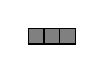
\begin{tikzpicture}[scale=0.1] \foreach \i in {2,4,6} \draw[fill=gray] (-1 + \i, 1) rectangle (1 + \i, -1); \end{tikzpicture} & \checkmark & \( {\{ \rightarrow, \acwopencirclearrow\}}^2 \) & Faster & Efficiency \\ \cmidrule{2-7}
				3G & \def\arcl{25}\multirow{3}{*}[-1em]{\begin{tikzpicture}
				\fill [gray] (0, 0) -- ++(-\arcl:1) -- (\arcl:1) -- cycle;
				\draw (0, 0) -- ++(-\arcl:1) (0, 0) -- ++(\arcl:1);
				\path (0, 0) [fill=gray] ++(\arcl:1) arc (\arcl:-\arcl:1);
			\end{tikzpicture}} & 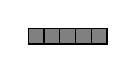
\begin{tikzpicture}[scale=0.1] \foreach \i in {2,4,...,10} \draw[fill=gray] (-1 + \i, 1) rectangle (1 + \i, -1); \end{tikzpicture} & \checkmark & \({\{\acwopencirclearrow\}}^2 \) & Faster & Efficiency, \$ \\ \cmidrule{3-7}
						4G &  & 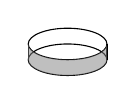
\begin{tikzpicture}[scale=0.4]
	\draw (0,0) ellipse (1.25 and 0.5);
	\draw (-1.25,0) -- (-1.25,-.5);
	\draw (-1.25,-.5) arc (180:360:1.25 and 0.5);
	\draw (-1.25,-.5) arc (180:360:1.25 and -0.5);
	\draw (1.25,-.5) -- (1.25,0);  
	\fill [gray,opacity=0.5] (-1.25,0) -- (-1.25,-.5) arc (180:360:1.25 and 0.5) -- (1.25,0) arc (0:180:1.25 and -0.5);
\end{tikzpicture} & \ccross & \( \acwopencirclearrow \)  & Less Moving Parts & More scattering \\ \cmidrule{3-7}

							H\gls{ct} &  & 3G/4G & 3G/4G & 3G/4G & Fast 3D & Bit more expensive \\ \cmidrule{2-7}
			MR\gls{ct} & \def\arcl{25}\begin{tikzpicture}
				\fill [gray] (0, 0) -- ++(-\arcl:1) -- (\arcl:1) -- cycle;
				\draw (0, 0) -- ++(-\arcl:1) (0, 0) -- ++(\arcl:1);
				\path (0, 0) [fill=gray] ++(\arcl:1) arc (\arcl:-\arcl:1);
				\draw [fill=gray] (0.9, 0) ellipse (0.1 and 0.43);
			\end{tikzpicture} & 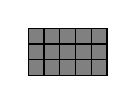
\begin{tikzpicture}[scale=0.1] \foreach \i in {2,4,...,10} \draw[fill=gray] (-1 + \i, 1) rectangle (1 + \i, -1);
\foreach \i in {2,4,...,10} \draw[fill=gray] (-1 + \i, -1) rectangle (1 + \i, -3);
\foreach \i in {2,4,...,10} \draw[fill=gray] (-1 + \i, -3) rectangle (1 + \i, -5);
		\end{tikzpicture} & \checkmark & \( {\{\acwopencirclearrow\}}^2 \) & Fast 3D & Expensive \\
			EB\gls{ct} & 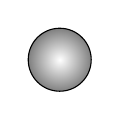
\begin{tikzpicture}
				\shadedraw[shading=radial, inner color=white, outer color=gray] (0, 0) circle (0.4);
				\end{tikzpicture} & 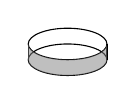
\begin{tikzpicture}[scale=0.4]
	\draw (0,0) ellipse (1.25 and 0.5);
	\draw (-1.25,0) -- (-1.25,-.5);
	\draw (-1.25,-.5) arc (180:360:1.25 and 0.5);
	\draw (-1.25,-.5) arc (180:360:1.25 and -0.5);
	\draw (1.25,-.5) -- (1.25,0);  
	\fill [gray,opacity=0.5] (-1.25,0) -- (-1.25,-.5) arc (180:360:1.25 and 0.5) -- (1.25,0) arc (0:180:1.25 and -0.5);
			\end{tikzpicture} & \ccross & None & Time Resolution & Expensive \\
			\bottomrule
		\end{tabularx}
		\begin{tablenotes}\small
		\item \checkmark\textsuperscript{*}: Narrow Beam (implicitly collimated), H:\@ Helical, MR:\@ Multiple Row, EB:\@ Electron Beam.
		\end{tablenotes}
	\end{threeparttable}
\end{table}
\begin{figure}
	\centering
	\begin{subfigure}{0.45\textwidth}
		\centering%
		\includestandalone[width=\textwidth]{\PFF{gen1}}
		\caption{First-Generation}%
		\label{fig:principles:scanner generations:1}
	\end{subfigure}\hfill%
	\begin{subfigure}{0.45\textwidth}
		\centering
		\includestandalone[width=\textwidth]{\PFF{gen2}}
		\caption{Second-Generation}%
		\label{fig:principles:scanner generations:2}
	\end{subfigure}\\
	\begin{subfigure}{0.45\textwidth}
		\centering%
		\includestandalone[width=\textwidth]{\PFF{gen3}}
		\caption{Third-Generation}%
		\label{fig:principles:scanner generations:3}
	\end{subfigure}\hfill%
	\begin{subfigure}{0.45\textwidth}
		\centering
		\includestandalone[width=\textwidth]{\PFF{gen4}}
		\caption{Fourth-Generation}%
		\label{fig:principles:scanner generations:4}
	\end{subfigure}\\
	\caption[Illustration of the principles of different scanner generations.]{%
		Illustration of the principles of different scanner generations.
		The different generations are discussed in detail in the text.
	}%
	\label{fig:principles:scanner generations}
\end{figure}
\paragraph{First Generation} First-generation scanners have the simplest geometry, which conceptually corresponds nicely to the mathematical theory of reconstruction discussed later.
Specifically, they consist of a single collimated (i.e.\ \enquote{pencil beam}) source along with a detector, that move linearly to acquire the attenuation along a line of a given angle.
After one such linear scan, the source-detector assembly is rotated incrementally, and continues to acquire the attenuation as described before, as illustrated in~\cref{fig:principles:scanner generations:1}.
Since the source and the detector move along a linear path (as opposed to, e.g.\ a fixed detector array), an arbitrary number of rays can be acquired.
Analogously, the angle increment may be chosen arbitrarily small, such that one can freely choose the number of projections.
This geometry further has the obvious benefit of conforming fully to the narrow beam geometry, i.e.\ the detected intensity only depends on the tissue along the path of the ray.
The obvious disadvantage of this simple approach is the slow speed, which is why they are not used in clinical practice today.
\paragraph{Second Generation} Second-generation scanners improve upon this by introducing a linear detector array (\cref{fig:principles:scanner generations:1}), such that one \enquote{fan beam} is measured simultaneously.
Still, the fan beam is not wide enough to cover the full field of view.
Initially, the opening angle of the fan beam was about \SI{10}{\degree}, consequently linear motion of the source-detector pair was still needed.
The detector array greatly reduced the acquisition time at the cost of abandoning the narrow beam geometry, such that detector collimation was needed.
By design, detector collimation reduces efficiency, such that for a given dose and identical projection measurements, a first-generation scanner would yield a better image.
However, the win in reduced acquisition time greatly outweighs the drawbacks of reduced efficiency.
\paragraph{Third Generation} Lots of scanners manufactured today utilize the general principle of third-generation \gls{ct} scanners.
Compared to second generation scanners, the opening angle of the fan beam grew to \SIrange[range-phrase=--]{40}{60}{\degree} (see~\cref{fig:principles:scanner generations:3}).
This means that linear motion is no longer necessary, as the fan beam can cover the full field of view.
Similar to the leap from first to second-generation scanners, the acquisition time is greatly reduced, but again the efficiency of the detectors is lowered.
This is necessarily the case, as without any linear motion the detector array must be very densely packed to obtain a sufficient number of samples per projection.
This requires the detectors to be very small, leading to some loss in efficiency.
Along with the number of detectors also increases the price of the system.
\paragraph{Fourth Generation} In terms of image quality and acquisition time, fourth-generation scanners do not have any advantages over third-generation scanners.
The difference lies in construction:
As shown in~\cref{fig:principles:scanner generations:4}, fourth-generation scanners utilize a stationary (i.e.\ non-rotating) \SI{360}{\degree} detector array, with only the \xray\ source rotating.
Since the detectors need to acquire signals from many positions, they can not be collimated.
Along with the possibility for physically larger detectors, this increases the detection efficiency as compared to third-generation scanners.
However, the interference of scattering events does not allow better image quality.
Such systems may be made more compact by positioning the source outside of the detector ring.
To allow the detectors to \enquote{see} the source, the detector ring may experience out-of-plane nutation out of plane.
Another possibility is to introduce gaps between the detectors to allow the \xray{}s to pass through.
We proceed by discussing classes of scanners with distinct characteristics, however, we do not assign a particular generation number.
\paragraph{Helical \gls{ct}} With the previously discussed scanner generations, exactly one slice of the body can be reconstructed during one acquisition run.
Typically, the slice thickness ranges from \SIrange{2}{5}{\milli\meter}, and in order to acquire three-dimensional datasets, one would have to move the patient with respect to the detector ring by this distance.
Clearly, this has the problem of being time consuming and prone to motion or misalignment artifacts.
The obvious solution to this problem would be to slide the patient through the tube whilst it is rotating around the patient, acquiring data continuously.
This is exactly the idea of helical \gls{ct} scanners, which otherwise do not differ from third or fourth generation scanners.
With this, it is possible to acquire full three-dimensional torso scans in around \SI{30}{\second}.
Today, most systems are capable of helical acquisition, as they are only marginally more complicated in terms of hardware, and the reconstruction problem (whilst seemingly much more complicated) can be solved with simple interpolation techniques.
\paragraph{Multiple Row Detector (Cone Beam) \gls{ct}} It is natural to extend the detector array into the second dimension to get a detector matrix.
Analogously to the detector array, the fan beam is extended into the third dimensions, such that multiple (these days up to \num{320}) one-dimensional projections are acquired simultaneously.
In some scanners, the array may be as high as it is wide, resulting in what is called \emph{cone beam} geometry.
If there is adequate distance between the \xray\ source and the detectors, approximately parallel planes can be imaged simultaneously.
Combining this with helical scanning allows to acquire full three-dimensional datasets to be acquired in the order of seconds, with reduced dose compared to conventional helical systems.
\paragraph{Electron Beam \gls{ct}} Up until now, all the discussed scanner geometries relied on one \xray\ source.
To get a full data set of one slice, this source (possibly also the detector array) has to be rotated around the patient.
Due to the heavy construction, one rotation of the \xray\ tube along with the detector array or matrix usually takes around one second (although, as discussed above, multiple slices may be acquired during this time).
This severely limits the ability to image (even a single slice) with high temporal resolution, e.g.\ for cardiac imaging or for tracing a contrast agent.
For this purpose, electron beam scanners have been developed.
These scanners produce the \xray{}s by an electron beam steered by electromagnets, which hits a stationary tungsten anode ring.
The resulting \xray{}s are detected by a stationary detector ring.
Since the electron beam can be steered very quickly (compared to the mechanical rotation of the tube-detector assembly), single-slice imaging can be done with a temporal resolution of about \SI{50}{\milli\second}.
\paragraph{Dual Source \gls{ct}} Dual (or multiple) energy \gls{ct} can be easily acquired with traditional scanner geometries by simply running multiple scans or pulsing different tube voltages.
However, this increases scan time and comes with other technical challenges, such that it is usually not done in clinical practice.
To overcome these issues, dual source \gls{ct} systems have been introduced, which operate with two physical tubes that allow different tube voltages.
Multi-energy imaging is desirable because of diagnostic benefits:
For instance, the composition of bones in the diagnosis of osteoporosis can be determined by such studies.
\end{document}
